% @Author: AnthonyKenny98
% @Date:   2020-02-23 14:27:21
% @Last Modified by:   AnthonyKenny98
% @Last Modified time: 2020-04-09 22:21:45

\subsection{Proposed Solution}
\todo[inline]{Revise and Rewrite}
    This thesis proposes a non-standard RISC-V Instruction Set Extension, supported by a functional unit embedded in a \gls{FPGA} synthesizable processor design that more rapidly computes motion planning for autonomous \gls{UAV}s. It will use the \gls{RRT} algorithm as a benchmark for performance analysis. Profiling of \gls{RRT} described in chapter \ref{chap:MotionPlanningInSoftware} found that edge collision detection was the most performance limiting function of \gls{RRT}. As such, this thesis aims to design a RISC-V extension and specific circuitry that support the faster execution of edge collision detection.

    \subsubsection*{System Overview}
        Figure \ref{fig:systemDiagram} shows a high level overview of the system this thesis proposes.
        % @Author: AnthonyKenny98
% @Date:   2020-03-01 11:14:04
% @Last Modified by:   AnthonyKenny98
% @Last Modified time: 2020-03-01 11:45:10
\begin{figure}[H]
\begin{center}
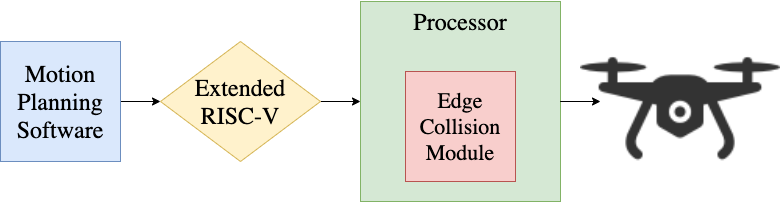
\includegraphics[width=\linewidth]{chapters/chapter1/img/systemDiagram.png}
\caption{System Diagram of Overall Project}
\label{fig:systemDiagram}
\end{center}
\end{figure}
        The \textbf{Extended RISC-V \gls{ISA}} is made up of the \gls{RV32I} Base Instruction Set and a \ifdraft{\color{red}\textbf{currently unnamed}\color{black}} non-standard extension that this thesis will define.
        The \textbf{PhilosophyV Processor} is a RISC-V chip built in \gls{HDL} for this thesis. It implements both the \gls{RV32I} instruction set and the non-standard extension.
        The PhilosphyV Core includes, along with a baseline 5-stage processor implementation, the \textbf{HoneyBee} collision detection unit.
        A \textbf{C Implementation of RRT} is loaded into the instruction memory of the PhilosophyV processor. This processor, synthesized on an \textbf{\gls{FPGA}}, is used as the main processor, co-processor, or accelerator on an \textbf{Autonomous \gls{UAV}}. Table \ref{table:componentList} outlines the components of this system and their descriptions.
        % @Author: AnthonyKenny98
% @Date:   2020-03-01 12:32:47
% @Last Modified by:   AnthonyKenny98
% @Last Modified time: 2020-03-01 13:59:51
\begin{table}[H]
\begin{center}
\begin{tabular}{|p{.2\linewidth}|p{.2\linewidth}|p{.5\linewidth}|}
    \hline
    \textbf{Component}          & \textbf{Source}   & \textbf{Description} \\
    \hline
    \multicolumn{3}{|c|}{RISC-V Instruction Set} \\
    \hline
    \ac{RV32I}              & Berkeley & 40 Instructions defined such that \ac{RV32I} is sufficient to form a compiler target and suport modern operating systems \cite{Waterman2019}. \\
    \hline
    Extension        & \textit{New} & This is the custom extension defined by this thesis targeting motion planning instructions. It is outlined in Chapter \ref{chap:RiscvProcessor}. \\
    \hline
    \multicolumn{3}{|c|}{C-Implementation of RRT} \\
    \hline
    RRT        & \textit{New} & Due to lack of available implementations of \ac{RRT} suitable for the purposes of this thesis, \ac{RRT} was implemented from the ground up in C. This is detailed in Chapter \ref{chap:MotionPlanningInSoftware} \\
    \hline
    \multicolumn{3}{|c|}{FPGA Synthesized Chip} \\
    \hline
    Zynq-7000        & Xilinx & The Zynq-7000 family of \ac{SoC}s are a low cost FPGA and \ac{ARM} combined unit. \\
    \hline
    PhilosophyV     & \textit{New} & The processor built for this thesis to demonstrate how the RISC-V extension and hardware unit work together. This is detailed in Chapter \ref{chap:RiscvProcessor} \\
    \hline
    HoneyBee        & \textit{New} & The functional unit designed specifically for faster execution of edge collision detection computations. Outlined in Chapter \ref{chap:MotionPlanningInHardware} \\
    \hline
\end{tabular}
\caption{List of System Components and their Descriptions}
\label{table:componentList}
\end{center}
\end{table}

    \todo[inline]{Update Above Table}

\subsection{Project Specifications}

    \todo[inline, caption={Project Specifications}]{This can just be the stuff from the start. Objective and 4 goals}

\subsection{Project Structure}
\label{subsection:project_structure}
    This report is structured to follow the timeline of this project, and is outlined below:
    \begin{enumerate}
        \item A benchmark motion planning algorithm, \gls{RRT}, was selected and implemented in software. Once implemented, a variety of performance analysis methods were used to profile the computational hotspots of the algorithm. It was found that edge collision detection was the critical function limiting execution time. This process is detailed in Chapter 2.
        \item With edge collision detection having been identified as the critical function, the process of designing specialised hardware to execute this function began. The technical specifications, performance specifications, designs, build phases, measurement and analysis of this hardware unit is presented in Chapter 3.
        \item With the aforementioned functional unit's performance verified in simulation, the next step was to implement this in a processor. First, a baseline processor was designed and built for this project to implement a base RISC-V instruction set. The performance of \gls{RRT} is again profiled on this baseline processor (as up until this point, it was profiled on x86 architecture). A non-standard extension to the RISC-V \gls{ISA} was then defined and support for this was implemented in the processor. Comparative performance analysis was then conducted. This process is described in detail in Chapter 4.
        \item Chapter 5 is a discussion of results and future work.
    \end{enumerate}

\todo[inline,caption={Summary of Results}]{Do I need a summary of results section in the introduction? }